\documentclass[a4paper, 12pt]{article}
\usepackage{amsmath}
\usepackage{listings}
\usepackage{amsfonts}
\usepackage{color}
\usepackage{graphicx}
\usepackage{float}
\usepackage{bbm}

\renewcommand{\thesubsubsection}{\roman{subsubsection}.}

\definecolor{dkgreen}{rgb}{0,0.6,0}
\definecolor{gray}{rgb}{0.5,0.5,0.5}
\definecolor{purple}{rgb}{0.5,0,1}

\lstset{basicstyle=\scriptsize\ttfamily,
breaklines=true,
language=Python,
showstringspaces=false,
keywordstyle=\color{blue},
commentstyle=\color{dkgreen},
stringstyle=\color{purple},
numbers=left,
numberstyle=\tiny\color{gray},
stepnumber=1,
numbersep=10pt,
backgroundcolor=\color{white}}

\title{Rechorder: A music prediction algorithm}
\author{Yash Savani (ysavani), Wilbur Yang (wilbury)}

\begin{document}

\maketitle

\section{Introduction}

For our project we wanted to predict the transitions that occur in music in real time. Our input is a midi file or a live stream from a midi instrument, midi is a well known and established format for music production and hence it was the obvioust choice. Our ouput is the predicted progression in the music. 

However, we did not want to classify music simply based on the classical chord progression given by western music theory. There are several examples of pieces that are played that do not follow the western chords (like indian classical music) and we did not want to leave these pieces out. Instead we chose to use an unsupervised learning algorithm to find clusters or motifs that were common among a certain genre of music, for instance in western music these motifs could represent chords. These clusters were determined by the note quality (frequency of the note), the length which the note was held down for and the dynamic range (loudness) of the note. 

Once we found the clustering of music using the unsupervised learning algorithm on a variety of different songs we wanted to predict how music progresses through these motifs. To do this we have decided to implement a range of models and supervised learning algorithms to find the best predictor for how music moves withing these motifs.
\section{Approach}

For our first milestone, we correctly found motifs and predicted the progression between the motifs using a simple Markov Model.

\subsection{Model}

We are modeling the problem in two parts: first, we cluster segments of the music files in our corpus, and then we look at the clusters as a Markov model or classification problem. The goal is to cluster similar chords together and then learn  when transitions between chord clusters occur, using machine learning. Here, when we say ``motif,'' we refer to variations of note groups which have the same base structure but may also have minor additions or deletions.

The clustering and classification training is all preprocessed so that when we run the program live, we can refer to the classification parameters to decide which chord cluster to transition to next, given the current music segment.

\subsubsection{K-Means Clustering}

To cluster the parts of a music file, we break the file into segments of four beats (see the assumption below), and we cluster those segments using K-means. We will refer to those segments as bars or motifs. Our aim is to cluster those bars into motif clusters to find general and popular motifs.

We work in the feature space that extracts, from a bar, the notes that are present and the percentage that each note is played in the bar. In particular, since we are dealing with music, we take the note value mod 12 as there are 12 notes in an octave (including sharps and flats) to normalize the pitch. Then, our feature vector is simply a mapping from a note to the percentage that is is played in the bar. We are currently measuring distances between feature vectors using the $L_2$ norm, but we are also looking into the cosine distance and other measures of distance, given that our feature space is $\mathbb{R}^{12}$.

The motivation behind this model was that each cluster centroid would represent a general feature vector for a set of similar motifs. We can then transition between clusters to get a progression of music.

\subsubsection{Classification / Markov Model}

We model the motif transitions as a Markov model, where each node is a cluster of motifs. The Markov model is trained by counting the occurrences of transitions between each cluster to each other cluster, and then taking the transition of maximum likelihood. We have implemented a working version of this, but we haven't gotten results for this yet. Using the Markov model, we should be able to transition from the current cluster to the next, given live music input.

We also plan on thinking about this part of the problem as a classification problem: classify a list of the previous few (perhaps 3 or 4) motifs seen as the next motif that we predict will occur. We have not implemented this idea yet.

\subsection{Assumptions}

We are segmenting the MIDI file into bars, assuming that each bar is comprised of four beats. This is a valid assumption for popular songs; most of these songs do not deviate from this time signature. We also assume that our corpus contains music with relatively similar styles and in particular does not contain any aberrant or discordant motifs.

\section{Results}

We have a k means clustering algorithm and a simple Markov model successfully working. 

\subsection{Testing model}
While we have successfully been able to test our algorithms on a small custom dataset we are in the process of building a much larger dataset and using k-fold cross validation to evalute our system. We have already built a scraper that scrapes for over 100 different midi files from http://midiworld.com and we have found a converter that converts all the midi files into midi format 0, with only one track that is required for our system. We will combine all the tracks and test on one tenth of the songs while training on the remaining and repeating the process for all ten tenths of the list.

Note that while we still have to implement this we do have successfully running models that have been evaluated using a smaller corpus of data.

\subsection{K-means}
To evaluate our results from the k means clustering and for feature selection, we used the average silhouette value. 

The silhouette value for a single example is the average distance of that point from another point that was classified into the same cluster times the minimum distance between the point to the centroid of another cluster divided by the maximum of the two values. The average silhouette value gives a good estimate for how well our clustering algorithm works within our dataset.

To find the optimal value of k, we ran k means 20 times on the input files using  
different values of k and plotted the results. The graph can be found below in fig 1. As we can see we found the optimal value of k to be 16. We plan on running it again with a larger maximum on k and with more midi files in the future.

Fig 1.
%\centerline{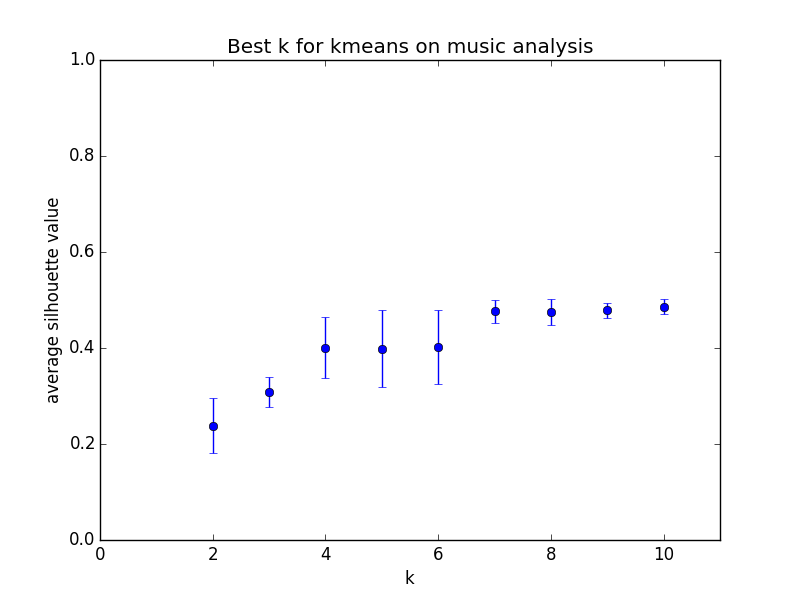
\includegraphics[width=10cm]{best_k_song_2.png}}

Our second figure (Fig 2) shows a visualization for the midi music and the clustering. The thick red horizontal lines indicate the music notes and the colored rectangles represent the cluster that the bars are in.

Fig 2.
%\centerline{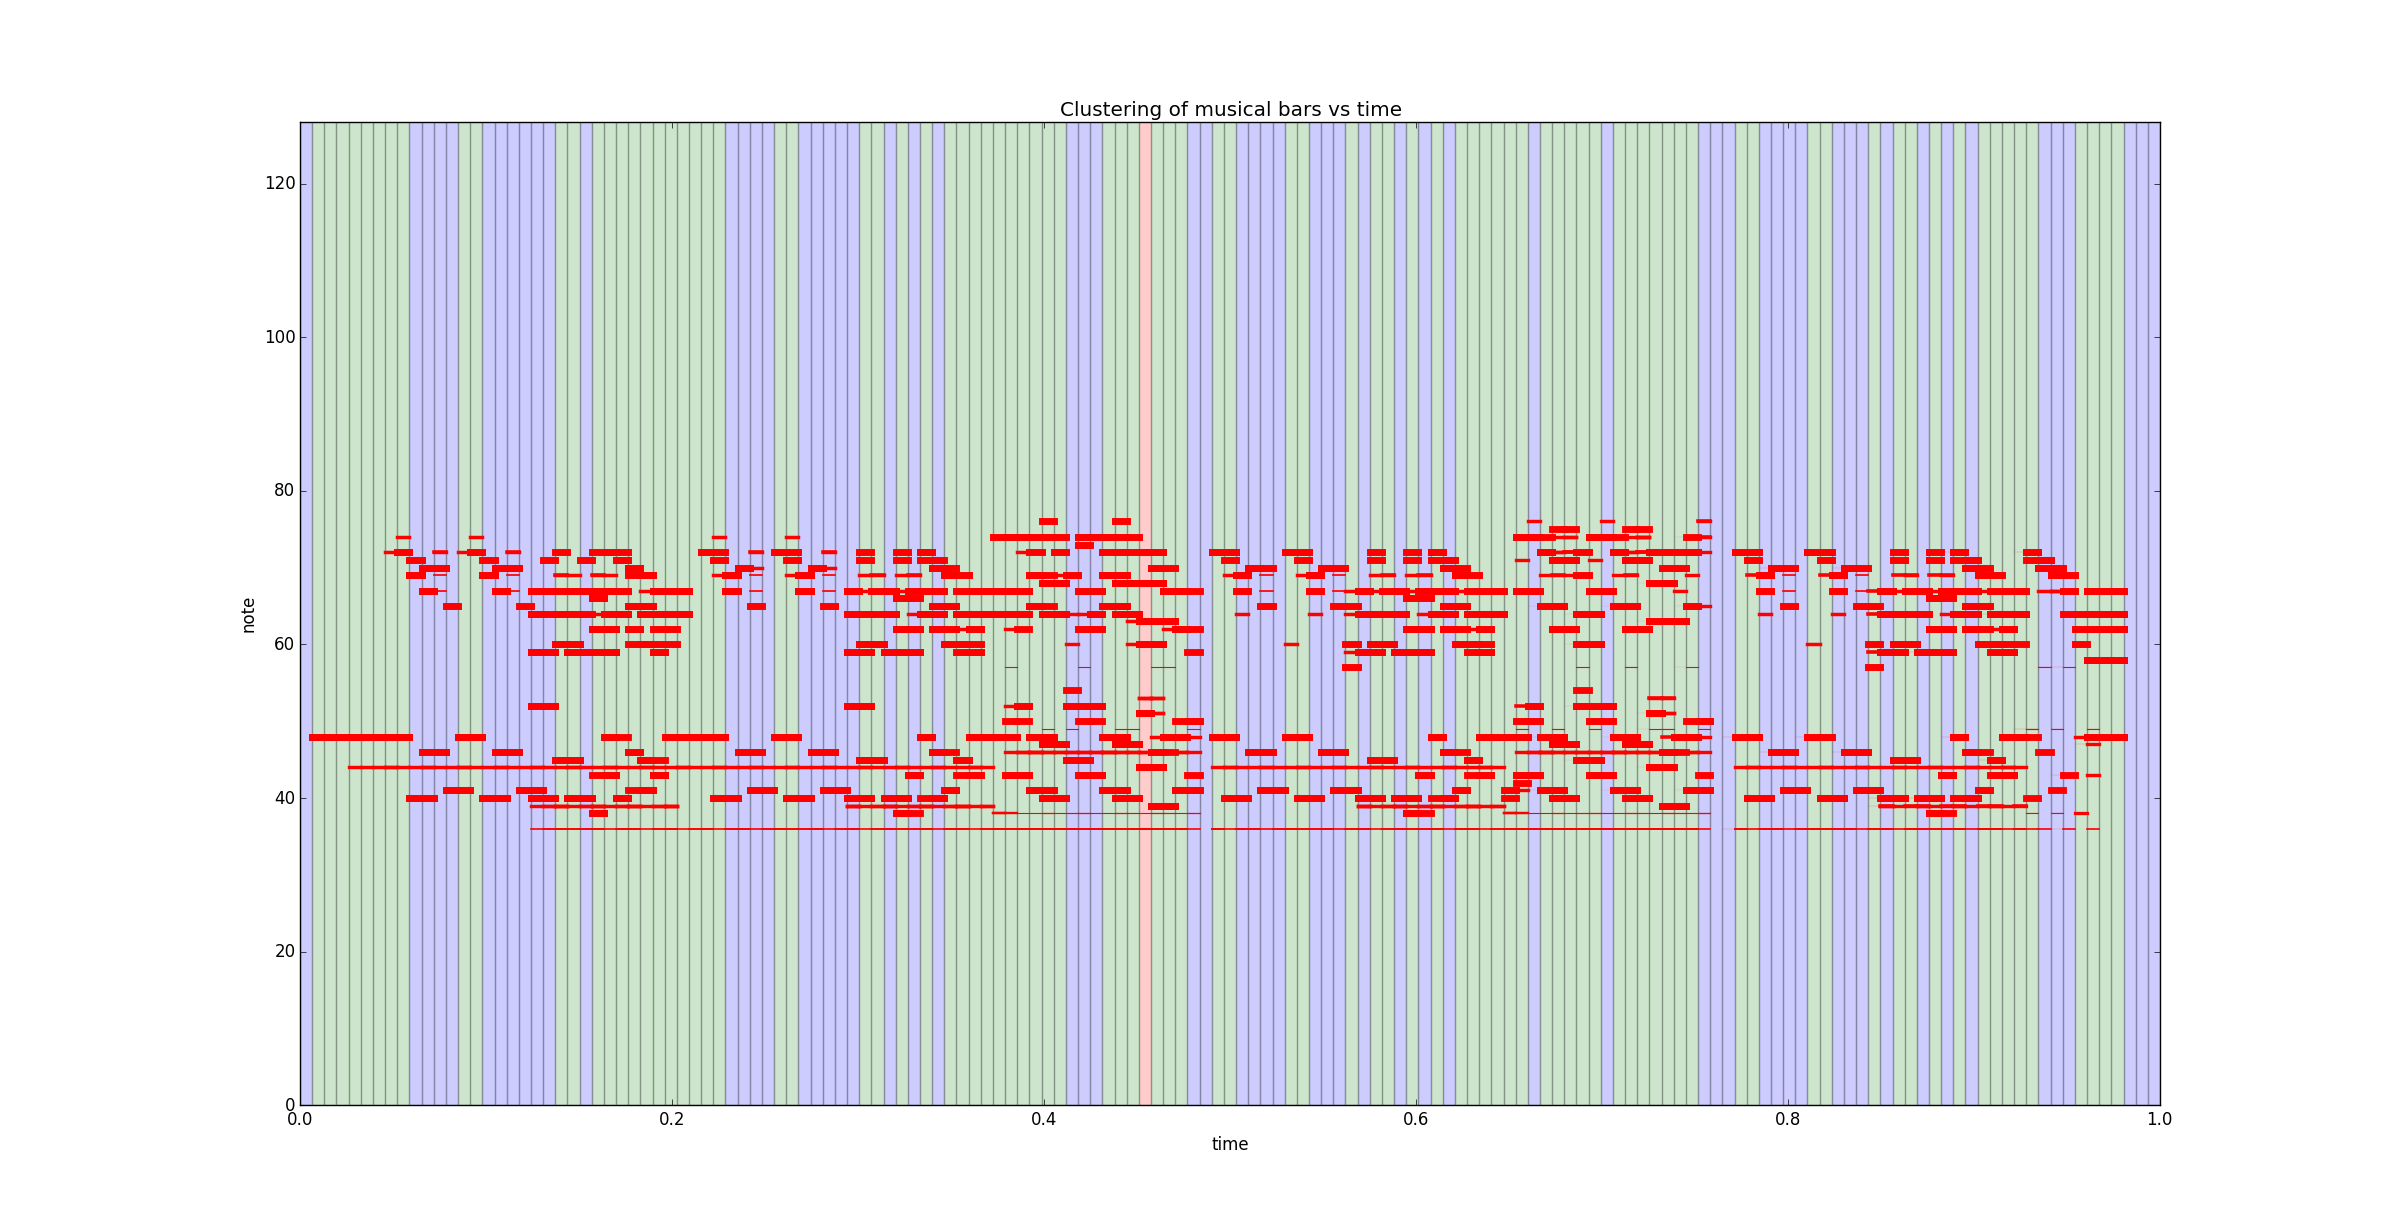
\includegraphics[width=10cm]{clustering_visualization.png}}


\end{document}